\documentclass[twoside,a4paper,openright,titlepage,draft]{ctexrep}
\usepackage[final]{graphicx}
\usepackage{subfig}
% \usepackage{subcaption}
\usepackage{extarrows}
\usepackage{multicol}
\usepackage{float}
\usepackage{amsmath}
\usepackage{subfig}
\usepackage{cancel}
\usepackage{wrapfig}
\graphicspath{{./pictures}}
\setcounter{secnumdepth}{3}

\begin{document}
\section{共栅极放大器}
\subsection{共栅极放大电路}
\begin{figure}[H]
    \centering
    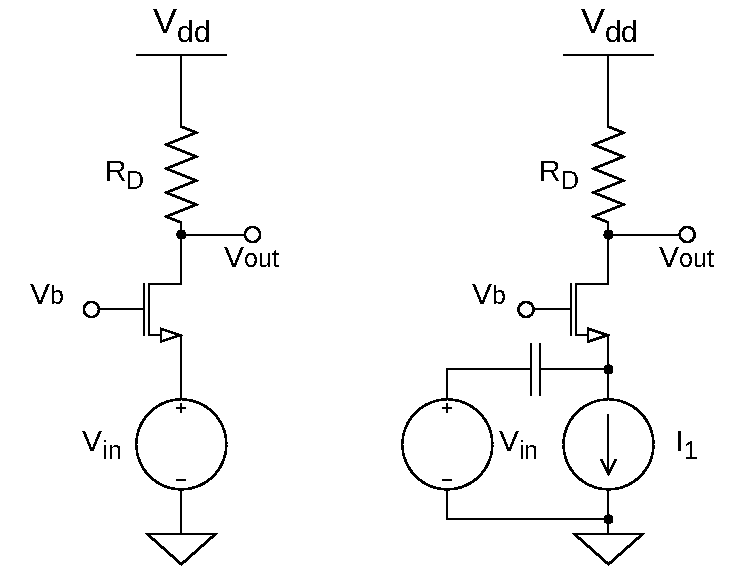
\includegraphics[height=60mm]{commongate.drawio.pdf}
    \caption{共栅极放大电路}
    \label{fig:共栅极放大电路}
\end{figure}
\subsection{工作区间}
只有当$V_{in}$足够小的时候,才能使管子导通:
\begin{equation}
    V_{in} \leq (V_b - V_{TH})
\end{equation}
这个时候直接进入饱和区。
\subsection{小信号增益Gain}
\paragraph{小信号模型图}
如图\ref{fig:小信号模型图}:
\begin{figure}[H]
    \centering
    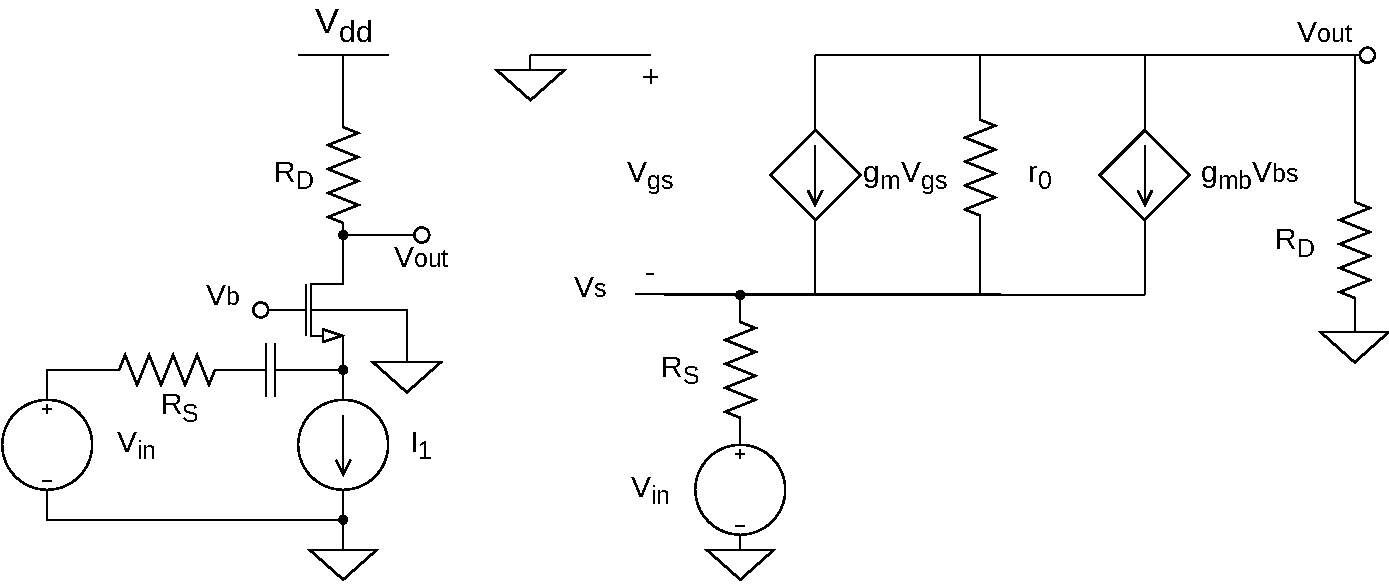
\includegraphics[width=\textwidth]{smallsignal.drawio.pdf}
    \caption{小信号模型图}
    \label{fig:小信号模型图}
\end{figure}
\paragraph{电压增益$A_V$}
\begin{align}
    A_V = \frac{v_{out}}{v_{in}} &= \frac{(g_m + g_{mb})r_0 + 1}{r_0 + (g_m + g_{mb})r_0R_S + R_S + R_D}R_D \notag \\
    &= \frac{(g_m + g_{mb})r_0 + 1}{[1 + (g_m + g_{mb} + \frac{1}{r_0})R_S]r_0 + R_D}
\end{align}
不用背,知道计算过程即可。
\paragraph{电流增益$I_{out} \over I_{in}$}
\begin{equation}
    \frac{i_{out}}{i_{in}} = \frac{R_S(g_m + g_{mb})}{1 + R_S(g_m + g_{mb}) + \frac{R_D}{r_0}}
\end{equation}
if $(g_m + g_{mb}R_S \gg 1)$:
\begin{equation}
    \frac{i_o}{i_i} \approx 1
\end{equation}
\subsubsection{小信号输入电阻}
\paragraph{小信号法}
如图\ref{fig:小信号测输入电阻}
\begin{figure}[H]
    \centering
    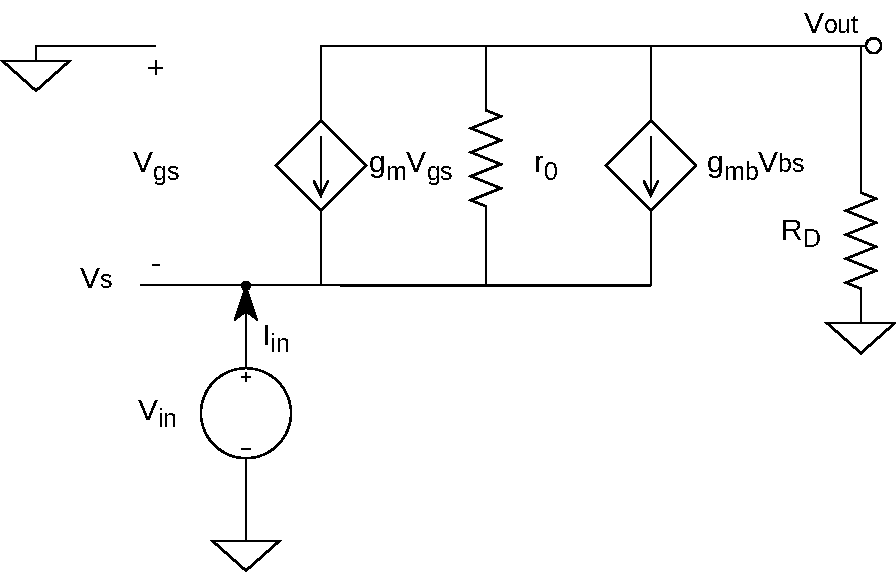
\includegraphics[width=0.66\textwidth]{inputimpedence.drawio.pdf}
    \caption{小信号测输入电阻}
    \label{fig:小信号测输入电阻}
\end{figure}
\begin{align}
    r_{in} = \frac{v_{in}}{i_{in}} &= \frac{R_D + r_0}{1 + (g_m + g_{mb})r_0} \\
    &\approx \frac{1}{(g_m + g_{mb})}(1 + \frac{R_D}{r_0}) \\
    &((g_m + g_{mb})r_0 \gg 1) \notag
\end{align}
结论:共栅极放大电路的输入电阻是一个很小的值。
\subsubsection{小信号输出电阻}
\paragraph{小信号法}
如图\ref{fig:小信号测输出电阻}
\begin{figure}[H]
    \centering
    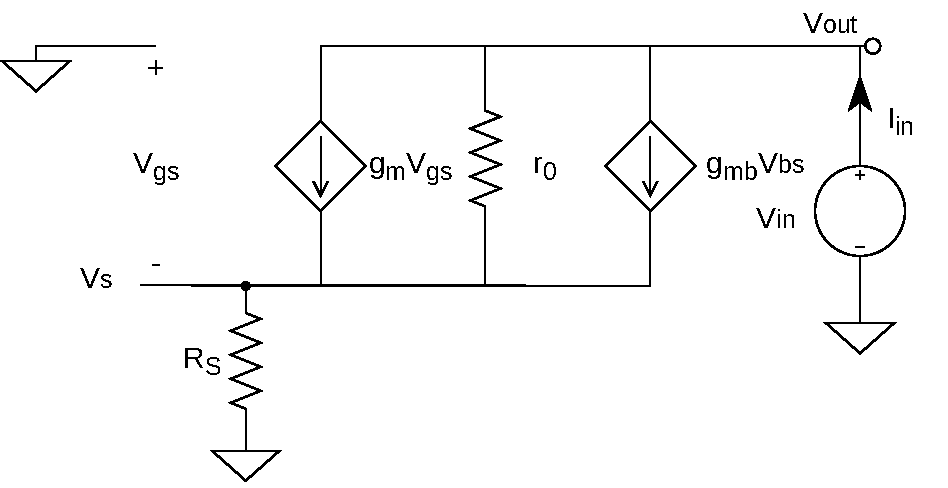
\includegraphics[width=0.66\textwidth]{outputimpedence.drawio.pdf}
    \caption{小信号测输出电阻}
    \label{fig:小信号测输出电阻}
\end{figure}
\begin{align}
    r_{out} &= [1 + (g_m + g_{mb})r_0]R_S + r_0 \notag \\
    &= [1 + (g_m + g_{mb} + \frac{1}{r_0})R_S]r_0 \\
    &[Very\ high\ if\ (g_m+g_{mb}R_S\gg 1!)] \notag
\end{align}
简化:
\begin{equation}
    r_{out} = g_mr_{0}R_S
\end{equation}
\subsubsection{Summary}
Common Gate电路具有:
\begin{center}
    \begin{enumerate}
        \item 很高的工作频率
        \item 很低的输入阻抗
        \item 很高的输出阻抗
        \item 将一个不够理想的电流信号变得更加理想
    \end{enumerate}    
\end{center}
\end{document}